In order to be able to write the program, we need to break down the problem into smaller problems, which are much easier to address, and link them together to create the final product.
\vs

I have created the following table highlighting the different sectors involved within the project.
\vs


\begin{longtable}{|p{4cm}|p{11.5cm}|}
    \hline
    Section & Purpose\\
    \hline
    \hline
    Base & This will contain the basics of the \m{Player} class, such as the hit-box, position, and collisions with the map.\\
    \hline
    Gameplay & Controls the length and state of the game, and will be responsible for display winners, managing teams and tracking player scores. Additionally, it will also control the game mode being played.\\
    \hline
    Weapon & This will have a base class and derived classes for individual weapons, and its methods and attributes, such as ammo, reloading, and weapon switching.\\
    \hline
    Database / Account Management & This will be done in SQLite as it is a lightweight database. Alongside this, a login system can be made, where the server is run on a web server. This is linked to the UI, which will allow users to enter their details and login.\\
    \hline
    UI & This will allow users to navigate the game, start games and login.\\
    \hline
    AI & A large part of the game will be AI. This will ensure that a player can join a game immediately and not have to wait for a queue. The player will be able to select different levels of difficulty.\\
    \hline
\end{longtable}
\vs

Here is a top-down diagram showing all of the different sections of the project. We will break down and discuss each section individually in depth, as well as justifying why these modules are necessary.

\begin{figure}[H]
    \centering
    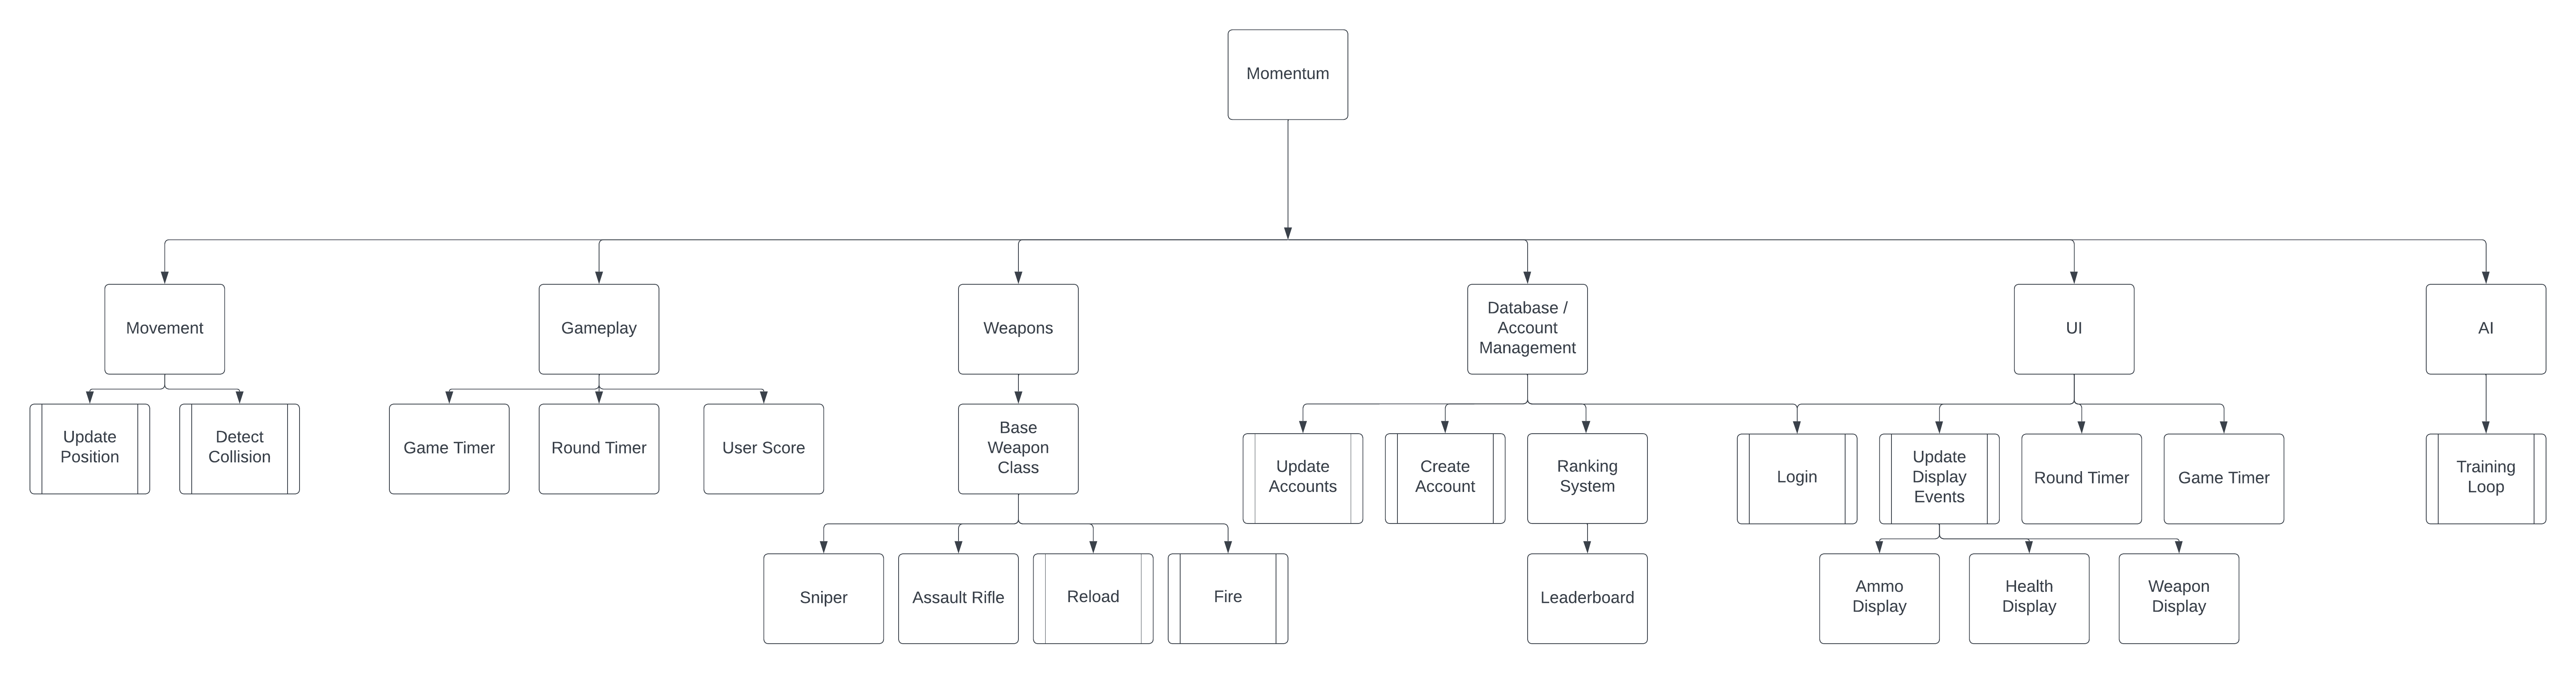
\includegraphics[width=15cm]{Design/Images/TopDownDiagram.png}
    \caption{A top down diagram of the project}
    \label{fig:td_diagram}
\end{figure}

In consideration of all these features there are few different languages and frameworks which come to mind as being suitable for the job. These are Unreal Engine, Unity, and PyGame. We will evaluate each one in turn.

\begin{longtable}{|p{2.8cm}|p{1.6cm}|p{5cm}|p{5cm}|}
    \hline
    Framework & Language & Pros & Cons\\
    \hline
    \hline
    Unreal Engine & C++ & \begin{itemize}
        \item Extremely performance orientated
        \item Supports OOP
        \item Has Learning Agents library (PPO)
    \end{itemize}
     & \begin{itemize}
        \item Not familiar with C++
        \item C++ is difficult to write and maintain compared to others
        \item Platform dependent
        \item Very hardware intensive
        \item Better suited to 3D games
    \end{itemize}\\
    \hline
    Unity & C\# & \begin{itemize}
        \item Also supports OOP
        \item Platform independence (bytecode)
        \item Implements MLAgents 
    \end{itemize} & \begin{itemize}
        \item Not familiar with C\#
        \item Lot of framework specific knowledge required
        \item Learning algorithm cannot be modified as much
    \end{itemize}\\
    \hline
    PyGame & Python & \begin{itemize}
        \item Very familiar with Python
        \item Many ML libraries in Python
        \item PyGame is much simpler than Unity and UE
        \item Platform independence
        \item Supports OOP
    \end{itemize} & \begin{itemize}
        \item Python is significantly slower than C++/C\#
        \item PyGame lacks lots of functionality that others provide
    \end{itemize}\\
    \hline
\end{longtable}

Based on all of these, I have chosen to go with PyGame for my project. 
\vs

\textbf{Justification:} This is because it provides the best flexibility and means that I do not have to work within the confines of a game engine that I am not as familiar with. This will allow for a much more controlled environment, and I have a lot of flexibility in how the game is implemented.

\vs
Additionally, PyGame is still relatively light, so despite Python being slow, it is possible to still get a 2D game running at 500-600 frames per second, and so even with more load placed on the system it should still be relatively quick.

\vs
One library that may be very useful to us, is \m{Cython}. This is a Python library which allows for Python files to be compiled into C, and then executed at runtime at a much faster speed thanks to C's performance.

\vs
However, this does have one caveat that the game code will have to be recompiled each time I want to make a change. Therefore, it makes the most sense to compile the game code at the very end when we have finalised all of the aspects of each class. This will provide a much more stable environment to work with and mean that I am not excessively recompiling each time I want to check whether a change has worked.


\tbr

\subsection{\textcolor{blue}{Game States}}

We will need several classes in order to run the game effectively. The first one is the \m{Game} class. This will control the whole application and contains the loop from which all other functions are called. This is justified because it allows us to encapsulate the entire application into one project, and we can have modules within it. It also makes certain things easier, such as managing all of the different states.

\vs
Then, we have the game state manager. This is effectively going to let us get and set which state we are in currently, and allows us to change it from within menus and other states. This makes it much easier to process and understand the game. This is justified because it gives us a centralised way to edit the current state in the game. This is useful because it means that we can move between states easily, and we can define this behaviour according to what we have done, just as clicking buttons in the menu, or pressing certain buttons.

\vs
\begin{longtable}{|p{3cm}|p{5cm}|p{7cm}|}
    \hline
    State & Explanation & Justification\\
    \hline
    \hline
    Start & This will be the main menu of the game, and will allow us to create a game, options, set timer, and exit game. & This is the main interface through which the user will interact with the game. Therefore, we need to have this in order to allow a user to intuitively interact with the game.\\
    \hline
    Options & This will be the options menu, containing things like keybindings. & This is important because it allows the users to customise the game to their standards and this makes it more enjoyable for the player, since it is to their liking.\\
    \hline
    Login & This will let a user who already has an account to submit their login credentials and will then verify these details. If they are valid, they are redirected to the start menu. & This is important because we need to have some way to track user progress in an accurate way, and so we also need to keep this in the game's state in some manner.\\
    \hline
    Register & If the user does not already exist, it will allow them to create a new account using an email address and password. & This will allow the user to be able to track their progress, which is quite important for some people, since it gives a sense of achievement.\\
    \hline
    Create Game & This will let the user create a game. & This is important since otherwise the main game loop would be inaccessible to the user, thus making my project redundant.\\
    \hline
    Set Timer & This will allow the user to set how long they would like to play for in the entire session. & This was one of the things that was mentioned by the stakeholders as being very important to the project.\\
    \hline
    Game Loop & This will be the place where the user will spend the majority of their time. This will run the main game and will be the main attraction of my project. & This is a game state because we need to be able to shift between this and the other game states and menus.\\
    \hline
    Game Over & Once the player's time is over, or the round is over, the user must either be forced to exit the game, or to start another round if they still have time.& This exists as it also shows the outcome of the game and provides a nice way of concluding the user's experience without making it too abrupt.\\
    \hline
\end{longtable}

We will need to pass values between the game states in order to allow things like global variables to exist in the game state. This will contain things like player settings, PlayerID, and the amount of time left until the game will close itself.


\vs
There are a few possible \textbf{data structures} that we could use to transmit return values between different states. These are dictionaries, classes, and lists (linked lists and arrays are modelled as the same thing in Python.)


\vs
We will be using a dictionary to transfer these return values, because this is the most convenient and versatile format that will allow us to transfer data between states in a way that is maintainable. The other options that we have available to us is a class or a list.

\vs

\subsection{\textcolor{red}{Game Loop}}

We need to create a base of the game loop and will house all of the mechanics which are relevant to the game, such as the time left in the round, the score of each player, the position of each player, etc. This is important since we need to be able to track all of these statistics as we will need to update the user's profile after the game is over.

\vs
Firstly, we will define the processes and events which take place in the game loop.

\begin{longtable}{|p{3cm}|p{6cm}|p{6cm}|}
    \hline
    Event & Explanation & Justification\\
    \hline
    \hline
    Movement & This will allow the player to move and control their character on the screen. The player will move relative to the world. & The game relies on players interacting with each other which is only possible if they are able to move. The AI will use this movement and input system to simulate a real player but this will be fed into the inputs for another instance of a character.\\
    \hline
    Time Tracking & We will show the amount of time left in the round, and how much time they have left in their play session. & This was one of the features that appealed to a lot of the people that I interviewed. Having this feature will let them control how long they are playing for and to not exceed that.\\
    \hline
    Score & This will be updated every time someone makes an elimination, or is eliminated. & This will be used to update the ranking rating at the end of the game, so is essential to track accurately. During training this will be used to monitor rewards to train the model.\\
    \hline
    Weapons & Will look for events to fire weapons, and will check for any intersections between rays and players. This will then be used to update the ammo of the player and the health of the player if one is hit. & This is essential to the game since we must be able to interact with other players, and eliminate them in order to move the game forward, and to allow players to gain a score.\\
    \hline
    Rendering & The player will need to be able to see their character and HUD, but this is not relayed to each of the bots, and so therefore, this needs to be done independently of the current game. In other words, we take input from the state of the map right now, but the player's view does not interfere with the game's progress. & If the user cannot see the screen, then they will be unable to play the actual game. Therefore, is essential that the game is rendered accurately and consistently.\\
    \hline
    Collisions & We need a way of reliably tracking where players and whether they are colliding with the map or not. & This is important since otherwise, the game would be very dull and this adds more complexity to the strategies possible.\\
    \hline
\end{longtable}

\vs
We will have the player on the centre of the screen. We know the dimensions of the screen we are drawing, so for efficiency, if a player is not within those dimensions, we will not draw them, but they will still exist. We can do this, by calculating their relative positions to the player, and then translating to this to where they should be on the screen. We can do this with the formula shown below.
\begin{align*}
    x_\text{screen} &= x_\text{object} - x_\text{player} + \frac{x_\text{width}}{2}\\
\end{align*}

A similar expression is produced for the $y$ direction. We can calculate these co-ordinates for each object and then rule out those where the $x$ or $y$ ordinate is not on the screen. In the initial parts of the game's development, we will ignore this, and just render the whole map.

\tbc

\subsection{\textcolor{blue}{Movement}}

In order to create forwards and backwards movement, we just simply apply a multiple of the forward vector to the character. When the player presses W they will be moved forward, and when the player presses S they will be moved backwards. This is justified as this is the standard for most modern games, and so will be what most people are familiar with, hence making the game easier to start learning.
\vs
\vs
In order to rotate the character, a mouse will be used and the position of the cursor from the character will determine the angle which the character faces. This is justified because this will be the only way of allowing the user to accurately rotate the character where they want, since the only other common input is a keyboard, but this has binary readouts which will not allow the user as much control as they would with a mouse, which provides a much more refined output. This is then the angle at which any shooting is done, and the movement vectors will stay consistent with the direction the player is facing. The player will see a rotated player, and the world will stay in the same direction on the screen. This is justified because it allows for a much more intuitive experience. 
\vs
\vs
We can find this angle using the following formula, where we use $(x_0, y_0)$ to find the centre of the screen, and $(x_1, y_1)$ to represent the position of the cursor. Then, the angle below the horizontal line is $\theta$. If $\theta$ is negative, this just represents it points above the horizontal line. We will not run the code if the cursor is at the centre since otherwise this would return an infinite value. In that case, we can manually deal with the cases. We can see that if the cursor is below the centre of the screen then we must point downwards, and vice versa. We can justify using this formula since it is optimal for our application, as it has a constant complexity, and other ways that are not formulaic must have a larger time complexity. In a game, optimisation and efficiency are very important and so it is key that we use this formula to reduce computation time per frame, which is essential, since we are going to be using this formula very frequently.
\vs
\vs
\begin{align*}
    \tan \theta &= \frac{y_1 - y_0}{x_1 - x_0}\\
\end{align*}

\vs
The shift button will be used to dash which will move the player very quickly across the map, and will be put on a cool-down. This will be done by adding a sudden acceleration to the character in the direction they are currently moving, and then removing this acceleration, and decreasing the speed drastically. This effectively creates the illusion of dashing or jumping which is what we want to achieve. This is a justified 
\vs
\vs
Additionally, we will need a procedure to calculate position. We will set an initial position for each player. This will be where they spawn into the game initial, and where they respawn after each death. We will need to create an initial direction vector as well, in order to preserve the orientation of the player relative to the map.
\vs
\vs
There are two aspects to the development of the game. The first is the underlying framework which handles the "back-end", such as physically moving the players on the map, firing projectiles, detecting collisions, and tracking scores. Then, we have another section which handles the user's point of view of the game, such as the menus, the camera which tracks the player's character, and the UI.
\vs
\vs
Hence, in the development, we must consider the back-end of the project first, since this will allow us to train AI, who don't have a front-end to the game. The reason for this will be shown in the AI section.
\vs
\tbr

\subsection{\textcolor{red}{Weapons}}

There will be one parent weapon class which will contain all of the common methods and parameters that each weapon will take, such as handling ray casting to detect collisions with objects, and then further to see whether damage should be dealt to it. From this, individual weapon classes will be created which will allow for individual weapon categories to be made and customised, which players will then be able to select at the start of a game.

\begin{enumerate}[label=\alph*)]
    \item Assault Rifle
    \item Shotgun
    \item Sniper Rifle
    \item Sub-machine gun
\end{enumerate}

The base class will be as follows.

\vs
\begin{tabular}{|p{4cm}|p{11.5cm}|}
    \hline
    Attribute & Purpose\\
    \hline
    \hline
    Direction Vector & This will be a unit vector pointing in the direction that the player is facing.\\
    \hline
    Ammo & We will store the maximum ammo in each cartridge and the current ammo. This will be deducted by one each time we fire.\\
    \hline
    Firing & Each time we fire the weapon, we will create a ray which can be traced to detect collisions with the enemy players.\\
    \hline
    Reloading & This will cause the weapon to be unable to fire a period of time, but refills the ammo in the weapon.\\
    \hline
\end{tabular}

\subsubsection{Firing Procedure}

We need to be able to fire a projectile in the direction of the weapon. We set the source to be the centre of the player. We will then create a sprite centred at the source and will have a constant velocity in the direction of the of the weapon (the player's forward vector).

\vs
We will need to create a way to detect collisions between rays and blocks and between rays and players. We will then take the closest of the two collisions to be the "dominant" collision, in other words the collision which we will need to focus on primarily. If this collision is with another player, we will need to check whether they are on the enemy team or not, and if they are then we need to deal damage and award some points to the firing player, and otherwise, we do nothing.

\vs

\subsubsection{Collision Detection}

As mentioned before we need a way to detect collisions between a ray and an object. There are multiple types of collisions that we need to be able to detect and handle. In this case, the primary one is a collision between a line and a circle. We will be using vectors in our program, since this will let us quickly and effectively find collisions and use vector methods and properties which are much easier to work with than Cartesian equations.


\tbc
\subsection{\textcolor{red}{Database / Account Management}}

To do this, there is a class in the Unreal Engine framework that will enable me to connect the game to a database. This will be stored on a central server so that no user can access it directly, and a login page will be created. This login page will take a user's player name and password, hash the password locally, and transmit this data to the server. This ensures that no plain-text passwords are being transmitted which improves security. The server will then check whether such a player exists and whether their password hash matches what is stored. If it is correct, then the user is sent to the main menu, where they will be able to select from different options.


\vs
The database is normalised to reduce data redundancy and maintain data integrity. It also allows for a more flexible structure and so should any new information or variables need to be stored we will be able to easily incorporate it into our database. We need to be able to hold the following fields as described by our success criteria.


\vs


\begin{longtable}{|p{3cm}|p{2cm}|p{9cm}|}
    \hline
    Field & Type & Justification\\
    \hline
    \hline
    Player ID & String & This will be part of what the user uses in order to login, and so therefore it also acts as a username of sorts. This will be linked to every bit of information about the user, which means that we can implement features showing the user statistics if they want to find out.\\
    \hline
    Email & String & This will let us create the account initially. Additionally, if the user needs to reset their password, then if they have their email they can get the game to send them an automatically generated password that they can change later.\\
    \hline
    Player XP & Int & This will be the basis for the level system in the game and will be one of the criterion for the leaderboard. The leaderboard will be a key feature of the game as it will add a sense of competition to the game for those that enjoy it.\\
    \hline
    Password & String & This will actually store the hash of the password, since storing the actual password in plain-text is extremely insecure, and will leave user details susceptible to being hacked. For example, if the database is somehow leaked, we don't also want it to mean that the passwords are all immediately revealed as well. However, we still need a secure way of authenticating users so that they can login, so the client version of the game will hash the password and then send a query to the server asking to verify the information.\\
    \hline
    Matches Won & Integer & One of the leaderboards will be based on the number of games won, and so therefore, we will need to store this information. Additionally, this might be one of the statistics that the users may want to know.\\
    \hline
    Matches Played & Integer & This is another thing which a player may be interesting in tracking. This will form part of the leaderboard as well.\\
    \hline
    Rating & Integer & This will be tracked and form another leaderboard and will give the player a larger sense of achievement and so encourages them to play more often.\\
    \hline
\end{longtable}

\vs
This gives us the following database structure.

\begin{figure}[H]
    \centering
    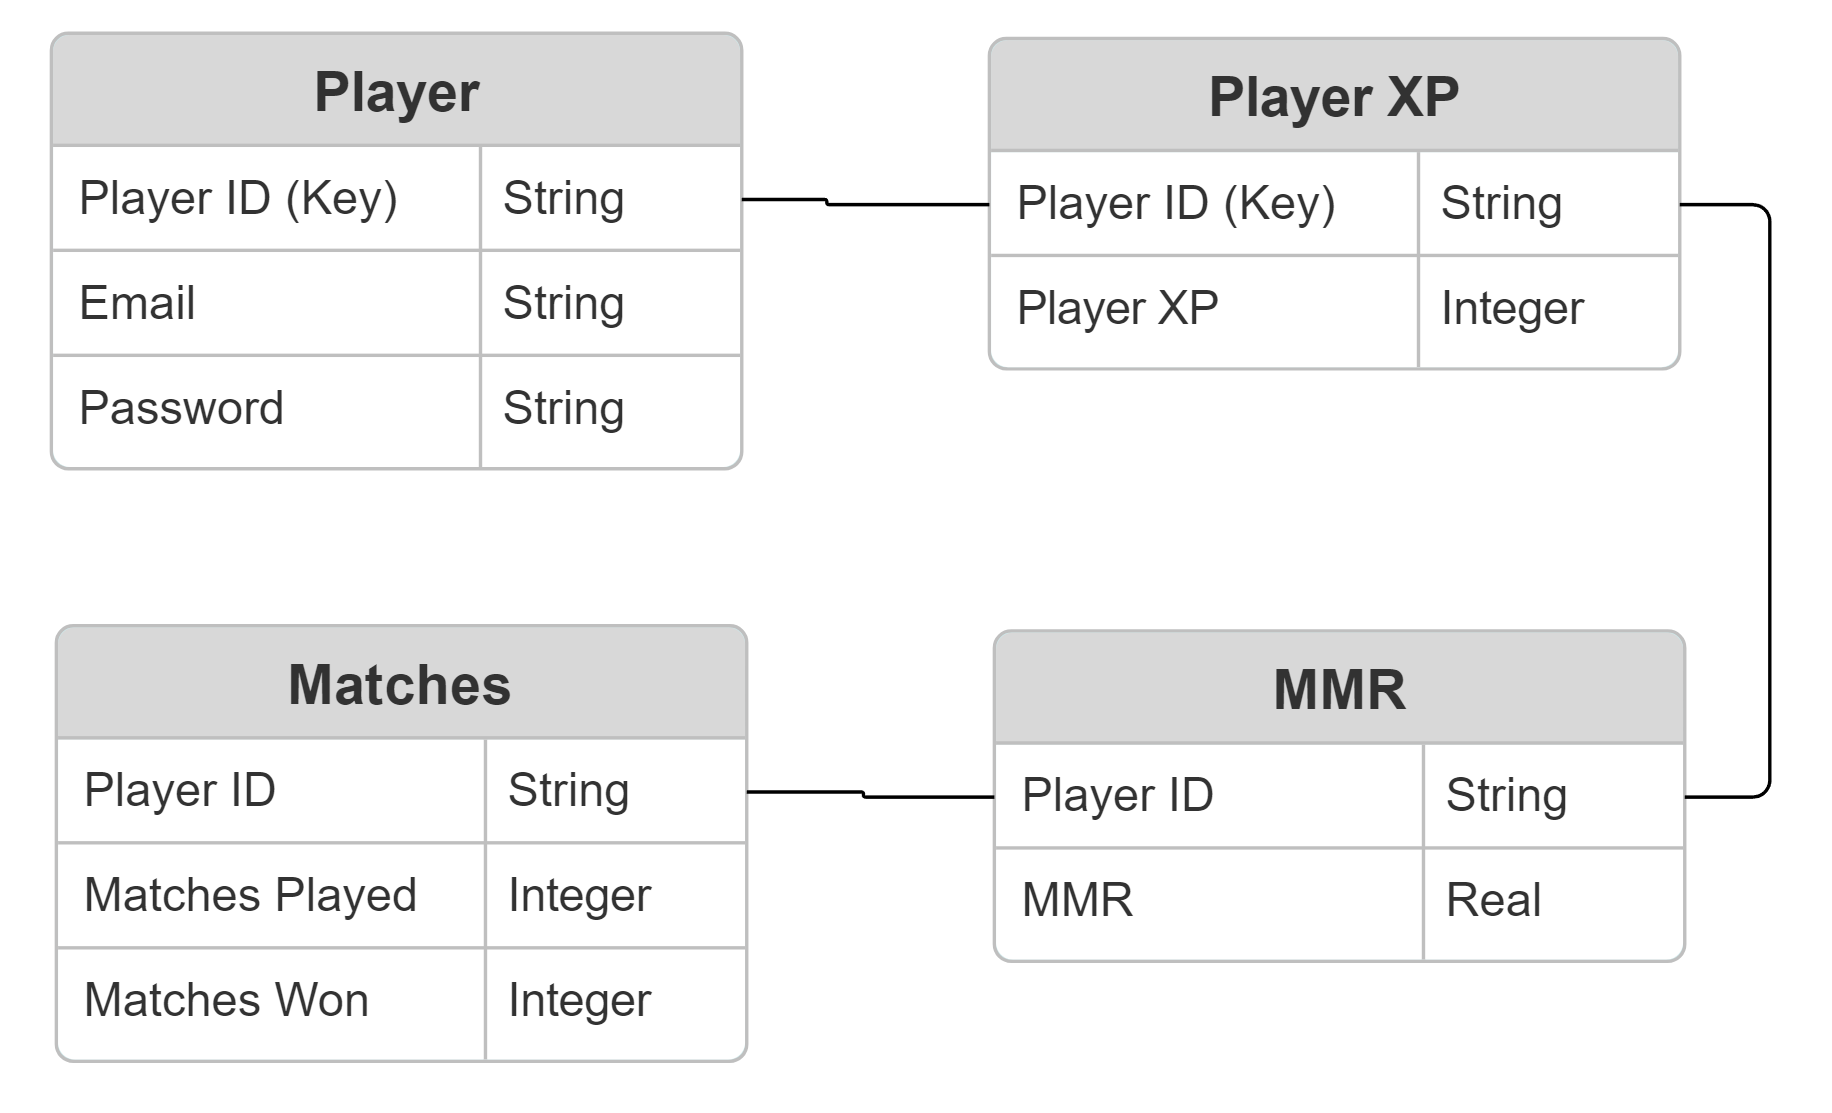
\includegraphics[width=15cm]{Design/Images/Database_Structure.png}
    \caption{An ER diagram of the database structure}
    \label{fig:db_structure}
\end{figure}

\vs
This database structure is justified because it is in 3NF. This means that we can query and search the database effectively and maintain referential integrity across the tables. We have chosen Player ID to be a key across the entire database because this will allow us to access all user information given the ID of the player. They will also be using this to login, and so we can quickly verify their login credentials when they are trying to login.

\tbc

\subsection{\textcolor{red}{UI}}

UI is essential to ensure that a user is able to quickly understand what each button does, and how to access what they need. For this reason, the only buttons present on the main menu will be "Play", "Settings", "Exit". This reduces any confusions that players may have, and allows the game to be much easier to pick up.

\vs
Here are some flowcharts detailing how the UI will lead to different sections of the game.


\vs

Additionally, we will now examine some different elements of the UI and justify why they are designed in a specific manner.

\vs
Firstly, I have chosen Iosevka as my font, as it is a sleek, modern font which I think is quite readable, but is very unique. This adds a unique element to the game.

\subsubsection{\textcolor{red}{Start Menu}}

The start menu will lead to the login menu, and so we really just want to provide a button for the player to click on. This is shown in Box INSERT FIGURE AND BOX NUMBER HERE.

The box will have a background colour which will be different to the rest of the screen in order to highlight that they can click there. This is important because usually in applications the cursor changes if you can click on something, however that is not the case here, and so we need to provide another way of conveying that information.

\vs
\subsubsection{\textcolor{red}{Login Menu}}

\vs
In the login menu, we want to allow the user to enter in their details and click submit to authenticate their account. This will be linked to the database handler, and so will need to provide the password to the database handler.



\subsubsection{\textcolor{red}{Main Menu}}

The main menu will house all of the other options that are available to the user, and so as shown in INSERT FIGURE AND DIAGRAM HERE, I have placed buttons adjacent to each other in a way that is intuitive.

\vs
Additionally, as seen in Box (INSERT BOX LETTERS HERE), we can see that there is still a background behind each box as explained previously.

\vs
Additionally, as shown in Box (INSERT LETTERS HERE), we can see the game's logo to create a sense of excitement, and since this is fairly common for games to do.

\subsubsection{\textcolor{red}{Set Timer}}

Here, we want to set the global timer, which will shut the game off after a game is finished. This will mean that we need to set a definite time limit as dictated by the user. We will also display the time at which the user's time will be over, so that they are aware of how long they have left.

INSERT DIAGRAM HERE

\subsubsection{\textcolor{red}{Create Game}}

In this menu, we want to be able to set the game's difficulty. This is done using arrows, since this seems to be the most intuitive way of doing something like this. Alternatively, a plus sign and a minus sign could be used also, since those explain more clearly what is going on.

INSERT DIAGRAM HERE

\subsubsection{\textcolor{red}{Game Loop}}

In the main game loop, we still have some UI elements to draw on. Primarily, we need to draw on the time as shown in Box INSERT BOXHERE, and we can draw other elements in a more clear way, such as by writing the amount of health each player has on the player itself, which quite clearly shows what is going on.

\vs

INSERT DIAGRAM HERE


\subsubsection{\textcolor{red}{Game Over}}

Once the game is over, we want to show the player where they have ranked relative to the other players.

INSERT DIAGRAM HERE

\subsubsection{\textcolor{red}{Leader Board}}


INSERT DIAGRAM HERE

\tbc

\subsection{\textcolor{red}{AI}}

I will be using PyTorch in order to handle the reinforcement learning aspect of the project. This is because it has extensive reinforcement learning tools, and is something which I am familiar with. Reinforcement learning works by using neural networks to create an output given a set of inputs. This is then processed and the action is taken. A reward is then assigned to this new state, and based on this, the model is adjusted through back-propagation and another step is taken. This continues millions of times, and this allows for the model to become progressively better. In order to create a game-like scenario, there will be 8 bots in two teams which will play against each other. The inputs to the bots are as follows, and all of this information will be condensed into a vector which is fed into the model.

\vs
\begin{enumerate}[label=\arabic*)]
    \item Current ammo - Provided as a real value between 0 and 1, denoting the proportion of ammo left, and computed by dividing the current amount of ammo by the ammo in a full weapon
    \item Current Health - Provided as real value between 0 and 1, and is computed by dividing the current health by the total health
    \item Distance to nearest health pad - This is given as a real value, and will be calculated using $r = \sqrt{(x_0 - x_1)^2 + (y_0 - y_1)^2}$, for the bot at $(x_0, y_0)$, and a health pack at $(x_1, y_1)$.
    \item Angle to nearest health pad - This is given as a real value, and can be calculated by $\arctan \frac{y_1 - y_0}{x_1 - x_0}$
    \item Spokes protruding from the centre of the players will extend to a set distance $r$, and will return 0 if there is no objects obstructing the spoke, will return $d$ if there is any enemy at distance $d$ from the centre of the player along that spoke, where $d<r$, and $-d$ if there is a wall obstructing the spoke at a distance $d<r$.
\end{enumerate}

\vs
The best model for this project is multi-agent reinforcement learning, as this will allow me to generate multiple bots which can compete against each other. Something like Deep Q Networks would not function in this environment because of the continuous nature of the game and the complex nature of the game.

\vs
The algorithm we will be using is Proximal Policy Optimisation, which relies on a clipped surrogate objective. This is an algorithm which can be expanded to a multi-agent version, which is what we want.

\vs
In order to do this, there will be a shared experience buffer, which will allow the agents to learn much faster than if they were playing individually. In order to allow the player to play, during the actual game, one of the agents will be "turned off", restricting the inputs that the AI gives, but still allowing the data buffer from the player to be transferred to the other two bots. This gives the game the feeling of playing with a team, rather than a more individual experience. This variant of the original Proximal Policy Optimisation which we will be using specifically, is known as MAPPO (Multi-agent Proximal Policy Optimisation) which uses centralised training, and decentralised execution. This is perfect for our situation, because, the player will not be able to communicate with the other bots during the game, and so it is ideal to have to have decentralised training and critics.

\vs
Additionally, during training, the rendering can be disabled, and the frame rate set to a very high value, in order to increase the speed at which the models can be trained. Because the model will progress from one frame to the next, the speed between frames can be altered without any consequence on the other bots on the team.

\vs
Furthermore, we will use a technique known as self-play. This is relevant since this is a competitive / co-operative game, we will put two separate versions of the model against each other. This will allow the model to play against "players" of it's own strength, and will produce better training results. Additionally, we don't have any ready-made players to play against, so this is our only option. We will initialise the model with random values to begin with, and will train it against itself in the first iteration. 

\vs
After this, we will take a snapshot of both agents, and then we will stop training the second agent, but keep updating the first one. With this, we can then train for a few more episodes and then take another snapshot of the agent. We will then sample the most recent models from the snapshot window and then train our agent against those. This will provide a way to train the AI against a wide variety of different agents which may have different ways of playing the game.

\vs
The first thing we need to in order to train the AI is to create an environment in order to train it. We will be using the \m{PettingZoo} wrapper to do this. This provides a strictly defined way of stating the game, using observation spaces, action spaces and rewards.

\vs
The observation space is the things which each agent can see. In the design section, we mentioned that each agent will have spokes which go out from the centre of the player. This will let the agents see the environment around them in a limited way.

\vs
The action space is all of the possible actions that the agent can take from any one state. The model will predict what it thinks is the optimal move to take from a given state depending on the observations that each agent can see.

\vs
The actions are then fed into the environment, and this is then used to move to the next time-step of the environment. With this, we can then return rewards, which are used to update the actor and critic networks. The reward is based on the actions of the player. For example, if the agent is able to eliminate another player, then this will result in a positive reward, but if the agent is shot, this will result in a negative reward.

\vs
The algorithm we will be implementing is known as MAPPO, which is the multi-agent variant of Proximal Policy Optimisation, which aims to optimise a surrogate objective function, but clips the maximum change that each time step can make to the actor and policy networks. This is in order to prevent large policy changes which could potentially damage the performance of the agent significantly. There are two networks used, the actor network, and the critic network.

\vs
Both networks use the same input, which is the observation for that time-step to generate an output. The actor outputs a vector which is the action which the agent will take in the following time-step. The critic network will output a single value, which is the predicted value of the state (or in other words, what it thinks the reward is going to be in that state).

\vs
From the original paper, we can see the process unfolding as follows. We firstly initialise our networks, and start a loop, and we can train for as long as we like. We then execute something known as a policy roll-out. This is effectively running our agent in the environment for a few time-steps, and recording the observations, actions, rewards and resulting states. This will allow us to gather information to train our network with. We also compute something known as advantages. Effectively, this gives us an idea of how much better off we are due to an action. We use a discount parameter and a GAE parameter.

\vs
On top of this, we will be using a library called \m{TianShou} which provides a high-level API on top of PyTorch in order to implement reinforcement learning algorithms. Additionally, it supports multi-agent reinforcement learning with heterogenous agents (agents which are not the same), and will allow us to do self-play to train the agents.

\vs


\subsection{\textcolor{red}{Utility Class}}

There are a lot of maths related functions which we will need to use particularly in detecting collisions with players, objects and rays. In particular we will need the following to be implemented.

\vs
We will first look at line-to-line collisions, since they underpin a large proportion of the game. Once, we can do line-to-line collisions we can also do line-to-rectangle collisions which are important for the weapon aspect of the game. We can derive a formula for how far along the ray the collision occurs. In the entirety of the game, we want to work with vectors and scales of 0 to 1 between the start and endpoints. Let us call these constrains $\vec{p_1}$ and $\vec{p_2}$ for line 1, and $\vec{p_3}$ and $\vec{p_4}$ for line 2. We first find a possible solution, then check that it the values that we have received are both between 0 and 1, since they are both bound segments.

\vs

\begin{align*}
	\vec{d_1} &= \vec{p_2} - \vec{p_1}\\
	\vec{d_2} &= \vec{p_4} - \vec{p_3}\\
	\text{Line 1: } \vec{r_1} &= \vec{p_1} + \lambda \vec{d_1}\\
	\text{Line 2: } \vec{r_2} &= \vec{p_3} + \mu \vec{d_2}\\
	\vec{p_1} + \lambda \vec{d_1} &= \vec{p_3} + \mu \vec{d_2}\\
	\vec{p_1} + \lambda(\vec{p_2} - \vec{p_1}) &= \vec{p_3} + \mu (\vec{p_4} - \vec{p_3})\\
	\begin{bmatrix} \lambda x_2 + (1 - \lambda)x_1 \\ \lambda y_2 + (1 - \lambda) y_1 \end{bmatrix} &= \begin{bmatrix} \mu x_4 + (1 - \mu)x_3 \\ \mu y_4 + (1 - \mu) y_3 \end{bmatrix}\\
	x_1 + \lambda (x_2 - x_1) &= x_3 + \mu (x_4 - x_3)\\
	y_1 + \lambda (y_2 - y_1) &= y_3 + \mu (y_4 - y_3)\\
	\lambda (x_2 - x_1) + \mu (x_3 - x_4) &= x_3 - x_1\\
	\lambda (y_2 - y_1) + \mu (y_3 - y_4) &= y_3 - y_1\\
    \begin{bmatrix} x_2 - x_1 & x_3 - x_4 \\ y_2 - y_1 & y_3 - y_4 \end{bmatrix} \begin{bmatrix} \lambda \\ \mu \end{bmatrix} &= \begin{bmatrix} y_2 - y_1 \\ y_3 - y_4 \end{bmatrix}\\
\end{align*}

\vs
We have arrived at a series of simulataneous equations. These can be easily solved with the \m{np.linalg.solve()} in NumPy, which means we don't have to solve it ourselves. However, this does have one restriction that the equations must be linearly indepenent. This just means that we need to check before hand what the determinant of the matrix is.
\vs

We also need to implement some more methods that are really important to the game and are going to be used repeatedly. These are addition, subtraction and the dot product. These are the most frequently used in vector equations and so are important to have implemented. This also gives us a quick way of finding the square of the magnitude of a vector by taking a dot product with itself.

\vs
In order to add or subtract two vectors, we can just take each element of the vector and add or subtract these elements to get our final result. Since all of our vectors are only having two dimensions we can just do this manually, or using list comprehension which is much more readable and easier to debug.

\vs
Furthermore, we need to have methods for collisions which we will be doing repeatedly throughout the game, and so this is best abstracted into the \m{Utility} class such that we can worry about other implementation details instead of re-coding the same methods over and over again.

\vs
In order to do this, we can split the collisions into a few main components. The first one is between two players. Since the players are rendered as circles, we can use this to find how to adjust the player positions.

\vs
Here is a diagram INSERT DIAGRAM HERE, showing two players overlapping. We can immediately see a few important details. The first one is that the distance between the two player's centres must be shorter than 2 times the radius of the player, since this will mean that the players are overlapping.

\vs
In order to resolve the collision, we need to move a player by an amount such that they will no longer be colliding, but just touching. Assuming that there is a collision, the derivation for the amount to the move the player by is as follows.

\begin{align*}
    TODO &= NOT+DONE+YET\\
\end{align*}

\vs
On top of this we need some way to handle collisions between lines and circles. This is because one of our primary success criteria was that there had to be weapons in the game, and that the user had to be able to shoot other players and that damage had to be processed.

\vs
During my research I found this method to detect a collision between a line and circle is two constraint points were used. This method involved computing multiple dot products until a quadratic equation was reached, and from there, it was just a simple comparision to find whether a collision had occurred.


\vs
Furthermore, since there will be blocks in the game, the player must not be able to pass through them and neither should any fired rays. In order to satisfy this, we need to consider two more types of collisions.

\vs
The first type is between a line and rectangle. This is quite simple, since we can just break a rectangle down into 4 lines and check for intersections with each one. We just want to find the intersection which is closest to the origin of the ray.

\vs
The second type of collision is between a circle and a rectangle. In order to do this, we need to find the point on the rectangle which is closest to the rectangle. In order to do this, I have referred to \cite{rectangle_circle_collision}, which explains in detail how this is handled.

\vs
This will then let us resolve the collision by moving it an appropriate distance.

\vs
Now that we have looked at how this works in theory, we should discuss how this works in implementation. In order to speed up the process as much as possible, I have considered other libraries to handle mathematical operations, such as adding vectors, dot products, matrices, etc.

\vs
The most popular scientific computing library in Python is \m{NumPy}, which provides a lot of different methods all written in native C code, and compiled providing extremely fast computations. However, there is one issue with this, in that in order to use \m{NumPy} methods we need to be working with NumPy objects. This is an issue because creating NumPy objects like arrays is incredibly slow, and therefore we will need to assess whether it is worth using this at all, since it is very plausible that casting to NumPy objects is slow enough to outweight the efficiency of using NumPy methods.
